% This is samplepaper.tex, a sample chapter demonstrating the
% LLNCS macro package for Springer Computer Science proceedings;
% Version 2.20 of 2017/10/04
%
\documentclass[runningheads]{llncs}
%
\usepackage{graphicx}
\usepackage[table]{xcolor}
% Used for displaying a sample figure. If possible, figure files should
% be included in EPS format.
%
% If you use the hyperref package, please uncomment the following line
% to display URLs in blue roman font according to Springer's eBook style:
% \renewcommand\UrlFont{\color{blue}\rmfamily}

\begin{document}
%
    \title{Solving a skill labyrinth using Reinforcement Learning with Unity ML-Agents and Curriculum Learning}
%
    \titlerunning{Comparing RL and Curriculum Learning using ML-Agents}
% If the paper title is too long for the running head, you can set
% an abbreviated paper title here
%
    \author{\textbf{Mario da Graca}}
%   \authorrunning{M. da Graca}
% First names are abbreviated in the running head.
% If there are more than two authors, 'et al.' is used.
%
    \institute{
        \textsl{
            Self-optimizing Systems\\
            Winter Term 2022/23\\
            University of Applied Sciences (HAW Hamburg)\\
            Berliner Tor 5, 20999 Hamburg\\
        }
    }
%
    \maketitle              % typeset the header of the contribution
%
    \begin{abstract}
        This project report examines curriculum learning in Unity ML-Agents using a 3D skill labyrinth as an example.
        The task involves tilting the board on two axes to guide a marble through a labyrinth, filled with walls and holes, through which the agent must steer the marble in order to follow the correct path and reach the end.
        The agent's performance was evaluated using two different approaches: standard reinforcement learning and curriculum learning.
        Curriculum learning involves starting the agent with simpler sub-tasks, and gradually increasing the difficulty over time.
        The paper covers the technical details of the project, including setup of the environment, tuning of parameters, reward engineering and performance analysis of the trained agent.

        \keywords{Reinforcement Learning \and Curriculum Learning \and Unity ML-Agents}
    \end{abstract}
    %! Author = mario
%! Date = 25.01.2023

\section{Introduction}\label{sec:introduction}
Machine learning (ML) is a subset of Artificial Intelligence (AI) that focuses on the development of algorithms and statistical
models that allow computers to learn from data and make predictions or judgments without being explicitly programmed.
Reinforcement Learning is a type of Machine Learning that focuses on teaching agents to make decisions in a given environment
by maximizing a reward signal.
It is a method for an agent to learn how to behave in a given situation by executing specific
actions and watching the rewards that the environment provides.\\
ML and RL are widely used in a range of applications, such as robotics, autonomous vehicles, finance, healthcare and games.
This report explores Reinforcement Learning in the latter one, by creating a complex and agility focused labyrinth environment,
that an agent has to successfully solve.
With the help of Unity's ML-Agents~\cite{juliani2020} a model is trained using the standard Reinforcement Learning and Curriculum Learning~\cite{narvekar_learning_2018} approach.
The goal of this project was to explore the process of an agent learning a fine motor task.
The following chapter will explain the setup of the board game in real life and as a game in the Unity engine~\cite{Haas2014AHO} to lay the grounds
for the third chapter, where the reinforcement learning aspects of this project are described.
The focus is on the environment and training setup, as well as the reward engineering.
In chapter four the used metrics are discussed and the results presented, in order to give a qualified statement in chapter five
about the performances and show where the process can be improved.
    %! Author = mario
%! Date = 30.01.2023


\section{Game Implementation}\label{sec:game-implementation}

\subsection{Game board}\label{subsec:game-board}
The basic setup of the game is simple, yet the hard parts lie in the way the game is played.
As shown in Fig.~\ref{fig:wooden_board} the game board is made out of wood and tilt-able on two disconnected axes.
This allows the player to move the marble around without direct contact, just by leveraging gravitation.
The goal of this game is to reach the end on the right hand side of the board, without falling into a hole.
If the marble falls down, the player has to restart and is rewarded with the points that are associated with each hole.
To follow the rules, the marble has to pass the holes in the correct order given by the black line.
Only if these requirements are met, the player can win the game.
There is no time limit in this game.\\
The basic concepts are easy to learn, but solving the task is hard to master.
The game requires fine adjustments to the angles and quick reactions to prevent the marble from rolling uncontrolled through
the labyrinth.

\begin{figure}[h]
    \centering
    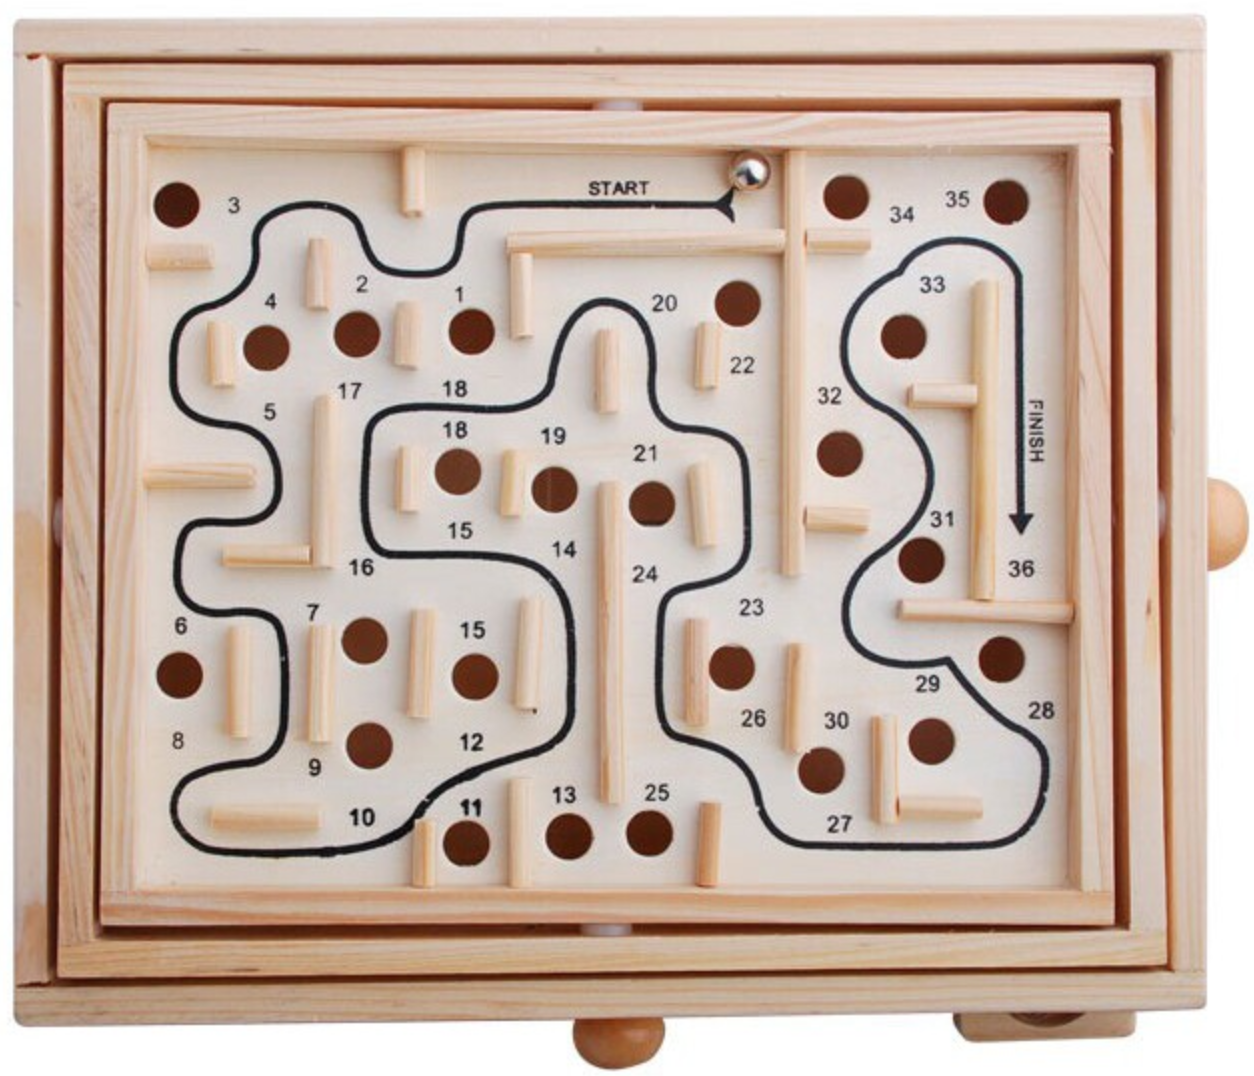
\includegraphics[width=0.65\textwidth]{images/wooden_game_board}
    \caption{The wooden game board, with the path to follow. Source:~\cite{wooden_board}}
    \label{fig:wooden_board}
\end{figure}

\subsection{Unity game board}\label{subsec:unity-game-board}
To closely approximate the movement and behavior of the marble in this physics based skill game,
Unity's built-in physics engine (PhysX3).
This system provides several components that can be attached to game objects, to ensure specific behaviors.
A game object in Unity defines the base for any entity in the given scene.
\begin{itemize}
    \item{Collider3D}: The Collider3D component can be added to any game object, either static or dynamic, to simulate the contact points of hard surfaces, like the marble or the game board.
    The shape is usually defined by or similar to the actual 3D model.
    This component can serve two purposes.
    It either behaves like a collider or, if specified by a flag, acts as a trigger, meaning it's not bouncing off other game objects.
    Instead it sends out a trigger signal.
    \item{Rigidbody3D}: To add game objects to the physics simulation that are affected by gravity, the Rigidbody3D component with the associated flag can be added to game objects with a Collider3D.
\end{itemize}
With these two simple components and a C\# script the controls and gameplay can be simulated.\\
In addition to the original game board, some modifications had to be made:
\begin{enumerate}
    \item{Top cover}: To make sure that the marble can't bounce out of the labyrinth, a transparent Collider3D has been
    added as a lid on top of the labyrinth.
    \item{Holes}: The board has holes in the base plate in the same positions as the original game board.
    Another Collider3D, but as a trigger, has been added below the game board to know, when the marble has fallen through a hole.
    The game will reset, if this event occurs.
    \item{Checkpoints}: Since the rules state that the marble has to follow the given path a checkpoint system has been implemented to ensure that the agent learns the correct behavior.
    A marble can only pass through the current checkpoint in line, otherwise the game will reset.
\end{enumerate}
    %! Author = mario
%! Date = 30.01.2023


\section{RL implementation}\label{sec:rl-implementation}

\subsection{Unity ML-Agents}\label{subsec:unity-ml-agents}
The Unity ML-Agents Toolkit is an open-source plugin for the Unity game engine.
It bundles easy to use functionality for environment creation, agent training, state-of-the-art RL algorithms and metric logging
all via the given Python API and Unity's editor interface~\cite{juliani2020}.
When working with this package there are only three main entities working together to build the training pipeline: Sensors, Agents and the Academy.
The Agent is the main component, it indicates that a game object serves as a trainable agent in the environment.
It can collect observations via different types of Sensors, take actions chosen by the policy and collect rewards to further improve its performance.
Possible types of observations are vectors of any length and any numerical datatype, images or ray-cast results.
The available RayPerceptionSensor casts rays from a specified point in any direction with an arbitrary length to determine distances to nearby game objects.
And lastly the Academy serves as the connection point, as it manages the simulation, its global steps and the agents in the environment.
The Academy can also be used to speed up the training process, by multiplying the training arenas in the scene, allowing a parallel training of agents on the same policy.
An experience buffer of specified size is filled up by all agents and once it's full the policy is updated.

\subsection{Basics}\label{subsec:basics}
The reason of this project is to compare the default reinforcement learning approach with the idea of curriculum learning.
Very hard or enduring tasks might take a long time for an agent to solve, hence the idea of splitting it into smaller subtasks seems obvious.
Curriculum learning is an extension to the widely used transfer learning in other Machine Learning areas~\cite{wiering_transfer_2012}.
Its goal is to create a series of source tasks for the agent to train on, such that the acquired knowledge
can be transferred to increase the learning speed and performance on the target task~\cite{narvekar_learning_2018}.
The major obstacle in using curriculum learning is building and choosing the subtasks~\cite{narvekar2016source}.
For this specific game three smaller sub-levels were created of the labyrinth~\cite{fig:unity_levels}.
The main idea is to train the agent on the whole labyrinth without holes first, to ensure that it is able to follow the specified path reliably.
In the following stages more and more holes are introduced, such that only small adjustments to the movements have to be made.
An agent advances to the next subtask, when it is able to solve the current task 100 times.

\begin{figure}[h]
    \centering
    \caption{Four stages of the labyrinth used for curriulum learning.}
    \label{fig:unity_levels}
\end{figure}

To train the agent the Proximal Policy Optimization (PPO)~\cite{schulman_proximal_2017} algorithm is used.
Since it's an on-policy algorithm that aims to find the best balance between exploration and exploitation, it's especially
well suited for this task in a continuous environment.
The alternative ML-Agents offer is is Soft-Actor Critic (SAC)~\cite{haarnoja_soft_2018}.
This approach is not used, as it is better suited for a sparse reward system, higher dimensional action space and heavier or slower
environments, with about 0.1s between steps, as suggested by Unity.

\subsection{Environment}\label{subsec:environment}

\subsubsection{Action Space}
The action space refers to the set of possible actions an agent can take in a given environment.
It is usually represented as a discrete or continuous space, where discrete actions are chosen as distinct elements
out of a finite set, whereas continuous actions are real-valued vectors, and in Unity's case are clipped between $[-1, 1]$.
As the controls of this game are fairly simple, so is the action space of this reinforcement learning task.
The size of the action space is set to two floats, meaning the Python API fills a buffer with two floats ranging between $[-1, 1]$ that will be converted into
the corresponding controls:
\begin{enumerate}
    \item{Rotation on X-Axis}: Rotates the labyrinth on the x-axis by the given amount in the action buffer multiplied with a constant rotation factor of 0.1.
    Depending on the sign of the action the board is either tilted towards positive or negative x.
    \item{Rotation on Z-Axis}: Rotates the labyrinth equivalent on the z-axis.
    Unity uses a left-handed, y-up coordinate system.
\end{enumerate}
Both actions are disconnected, meaning in one step the labyrinth can be tilted both on the x- and z-axis simultaneously.
By using a continuous action space the agent can tilt the game board more precisely, which results in finer control over the marble.

\subsubsection{Observation Space}
Contrary to the action space, the observation space describes the input of the agent, information that the agent receives from the environment.
It can also be discrete or continuous and is used to inform the decision making process of the agent.
The difficult trade-off is giving the agent enough data about it's surrounding to be able to converge on a good solution and not giving
too much irrelevant data, which slows down the learning process or could lead to suboptimal performances.
Agents in the ML-Agents package distinguish between two types of observations: vectors and images.
Images can be of arbitrary size with either grayscale or color information and vectors can be of any dimension with numerical values.
As mentioned above observations can also be collected off of Sensors like the RayPerceptionSensor, which yields information about
a ray-hit with another game object, like the normalized distance.
The best results were achieved with following set of observations:
\begin{itemize}
    \item{Rotation on X-Axis}: 4 floats represented as a quaternion
    \item{Rotation on Z-Axis}: 4 floats represented as a quaternion
    \item{Normalized Position of the marble}: 3 floats
    \item{Magnitude of Marble Velocity}: 1 float
    \item{Normalized Euclidian Distance to the next Checkpoint}: 1 float
    \item{RayPerceptionSensor Checkpoints}: A RayPerceptionSensor with 8 total rays around the marble to detect the next checkpoint
    \item{RayPerceptionSensor Holes}: A RayPerceptionSensor with 8 total rays around the marble tilted downwards to detect holes
\end{itemize}
This results in 13 float values passed in manually into the observation space buffer, with two added RayPerceptionSensors (16 rays)
automatically added by Unity.
Defining the observation space is a crucial step in developing a reinforcement learning game~\cite{song_observational_2019}.

\subsubsection{Reward Engineering}
Another very important step that determines the success of the learning process is the reward engineering~\cite{sutton_introduction_1992}.
Reward engineering describes the process of defining and shaping the reward signal, which is a scalar value that provides
feedback to the agent about its performance.
It indicates whether the actions it takes are good or bad.
A good reward function must accurately reflect the desired behavior of the agent, otherwise suboptimal or even
unwanted behaviors, that do not align with the intended task, can be the pursued by the agent.
There are two different ways of rewarding an agent in Unity's ML-Agents: explicit rewards and passive rewards.
With explicit rewards or punishments specific events are rewarded, meanwhile passive rewards encourage or discourage certain behaviors.
Both techniques are used for the skill labyrinth and are identical for both approaches, curriculum learning and normal learning.
During testing this step has gone through many iterations with vastly different reward functions.
The following set of rewards and punishments performed best in the scope of testing time in this project.\\\\
Positive rewards:
\begin{enumerate}
    \item Reaching the next checkpoint in line adds (+XXX * index of the checkpoint), encourages the agent to stick to the given path.
    \item To ensure that the agent doesn't steer the marble around too much, resulting in falling into holes or going the wrong way, the agent
    is reward the closer it gets to the next checkpoint (TODO: Formel).
    \item Reaching the goal adds (+1000.0)
\end{enumerate}
Negative rewards:
\begin{enumerate}
    \item Falling into a hole sets (-XXX). Ends the episode with a negative reward.
    \item Going through a wrong checkpoint sets (-XXX). End the episode with a negative reward.
    \item Analogue to the reward the agent is punished, if the marble is moving away from the next checkpoint or not moving at all.
    Adds (-XXX TODO:Formel)
    \item If the marbles velocity is below a certain threshold (XXX) for more than XXX steps, the episode resets with a negative reward (-XXX)
\end{enumerate}
This set of punishments and rewards was chosen based on the rules of the board game and the intended goal of the game:
Following the path to reach the end without falling into a hole.

\subsubsection{Hyperparameters}
Hyperparameters are parameters that are set before training and can not be learned from the data.
Unity ML-Agents offers a great flexibility by making all hyperparameters customisable.
This complicates the training process, since hyperparameter tuning is the main task in any Machine Learning application.
By observing the results and the training process, those parameters can be adjusted.
Doing this over and over again is a time consuming task, but it is necessary in order to achieve good results.
The following hyperparameters were tuned the most.\\
\textbf{batch\_size:}\\
The number of experiences (i.e.\ samples) to be used in each iteration of the training process.
Larger batch sizes can lead to faster convergence, but can also lead to slower training due to increased memory usage.\\
\textbf{buffer\_size:}\\
The maximum number of experiences to store in the experience replay buffer.
The agent samples from this buffer to learn from past experiences.
If the buffer size is too small, the agent may not have enough experiences to learn from.
If the buffer size is too large, the agent may waste memory on irrelevant experiences.\\
\textbf{lambd:}\\
A parameter used in the Generalized Advantage Estimation (GAE) algorithm~\cite{schulman_high-dimensional_2015}, which is used to calculate the advantages of actions in reinforcement learning.
The value of lambda determines the trade-off between bias and variance in the estimation of the advantages.\\
\textbf{hidden\_units:}\\
The number of neurons in the hidden layers of the neural network used for the policy and value function approximations.
Increasing the number of hidden units can result in a more complex model that fits the data better, but also increases the risk of overfitting.\\
\textbf{num\_layers:}\\
The number of hidden layers in the neural network used to approximate the policy and value functions.
Adding more hidden layers can increase the capacity of the model, allowing it to fit more complex relationships in the data.
However, adding too many hidden layers can lead to overfitting and slow down the training process.\\

\begin{center}
    \rowcolors{2}{gray!25}{white}
    \begin{tabular}{|c|c|c|}
        \rowcolor{gray!50}
        \hline
        \textbf{Hyperparameter} & \textbf{Normal RL} & \textbf{Curriculum Learning} \\ \hline
        batch\_size    & 2048      & 2048                \\ \hline
        buffer\_size   & 40960     & 40960               \\ \hline
        lambd          & 0.99      & 0.98                \\ \hline
        hidden\_units  & 1024      & 1024                \\ \hline
        num\_layers    & 3         & 3                   \\ \hline
    \end{tabular}
\end{center}
\begin{center}
    \vspace{10pt}
    \textbf{Tab. 1.} Used hyperparameters for normal RL approach and Curriculum Learning.
\end{center}
For the rest of the hyperparameters the default values were used.

\subsubsection{Training}
The concepts of reproducibility and determinism are critical in physics engines because they determine the accuracy and predictability of simulation results.
Reproducibility in a physics engine refers to the ability to obtain the same simulation results when run multiple times under the same conditions.
Determinism refers to the fact that, regardless of the hardware or software environment, simulation results should always be the same for the same inputs.
In the Unity game engine both concepts can't be fully guaranteed.
Trying to compare reinforcement learning with curriculum learning can't happen under fair circumstances, therefore both
approaches are run five times with the best set of hyperparameters, to compare a statistical average.
To reduce training time, the maximum number of steps was set to 75 million and concepts like parallel training were applied.




    %! Author = mario
%! Date = 07.02.2023

\section{Metrics and Results}\label{sec:metrics-and-results}
To compare different runs and both mentioned approaches three different metrics are evaluated.
The first is \textbf{episode\_length}, which represents the number of steps performed in a single episode, followed by \textbf{cumulative\_reward}, which is the sum of rewards collected over time, and finally the checkpoint index.
When the agent falls into a hole or passes through an incorrect checkpoint, the last checkpoint's index is logged.
For all of these metrics the average across all agents is calculated.
    \clearpage
    \bibliographystyle{splncs04}
    \bibliography{references}
%
\end{document}
